\documentclass[11pt]{article}
\usepackage[margin=1in]{geometry}
\usepackage{amsmath,amssymb,amsthm,mathtools}
\usepackage{graphicx}
\usepackage{microtype}
\usepackage{xcolor}
\usepackage[colorlinks=true,linkcolor=blue!55!black,citecolor=blue!55!black,urlcolor=blue!55!black]{hyperref}

\newtheorem{theorem}{Theorem}
\newtheorem{lemma}{Lemma}
\theoremstyle{remark}
\newtheorem{remark}{Remark}

\newcommand{\K}{\mathbb K}
\newcommand{\T}{\mathbb T}
\newcommand{\Id}{\operatorname{Id}}

\title{Square and Phase Norm Equalities on $C_0(L)$}
\author{Run \texttt{fa\_banach\_001}, lane 4\\Agent \texttt{agent\_lane\_04}}
\date{9 August 2026}

\begin{document}
\maketitle

\begin{center}
\fbox{\parbox{0.91\textwidth}{\textbf{Status.}
Candidate strong partial result, likely valid, pending human review.  The
packet completely classifies both real square identities and every complex
fixed-phase identity from the source on the classical spaces $C_0(L)$.  The
source's arbitrary-Banach-space questions remain open.}}
\end{center}

\section{Source questions}

Kadets, Mart\'{\i}n, and Mer\'{\i} study norm identities required of every
rank-one operator on a Banach space \cite{KMM}.  In the real case they say
that the nonsurjective analytic-function case is unclear and single out
$g(t)=t^2$ and $g(t)=-t^2$.  The resulting identities are
\begin{equation}\label{eq:squares}
 \|\Id+T^2\|=1+\|T^2\|,
 \qquad
 \|\Id-T^2\|=1+\|T^2\|.
\end{equation}
Their source Proposition 4.8 characterizes these identities geometrically,
but does not identify the spaces satisfying them.  In the complex case they
study, for $\omega\in\T\setminus\{1\}$,
\begin{equation}\label{eq:phase}
 \|\Id+\omega T\|=\|\Id+T\|
 \qquad\text{for every rank-one }T,
\end{equation}
and write that they do not know whether the infinitely many subgroup
properties are all equivalent.

\begin{figure}[ht]
\centering
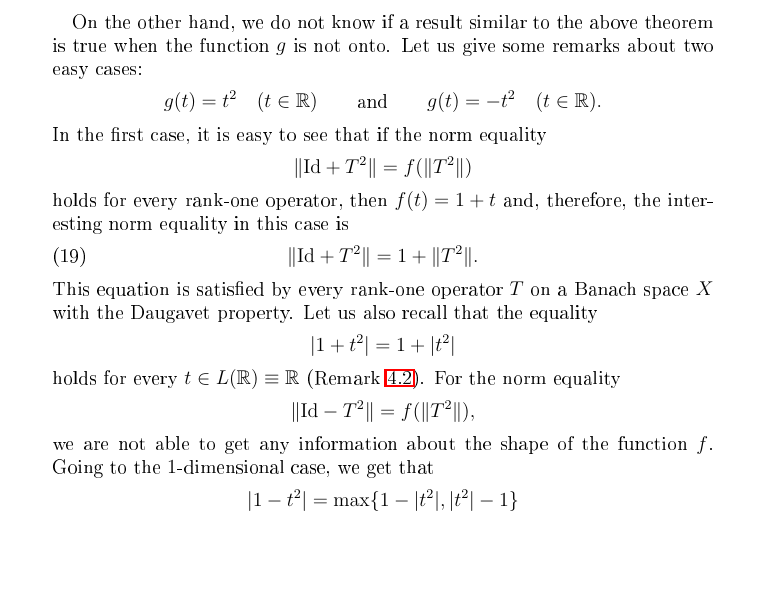
\includegraphics[width=0.92\textwidth]{figures/real_square_questions.png}
\caption{The real nonsurjective case and the two square identities in the
source PDF, pages 16--17.}
\end{figure}

\begin{figure}[ht]
\centering
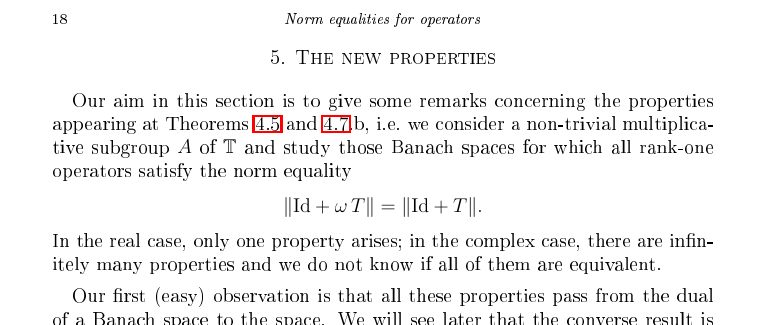
\includegraphics[width=0.92\textwidth]{figures/complex_phase_question.png}
\caption{The complex equivalence question in the source PDF, page 18.}
\end{figure}

The theorem below gives a complete answer to all these questions on real and
complex $C_0(L)$ spaces, equivalently on commutative $C^*$-algebras and
AM-spaces represented in this form.

\section{Classification theorem}

Let $L$ be a locally compact Hausdorff space and let $C_0(L,\K)$ carry the
supremum norm.  We exclude the one-point real space in the first statement:
there $T^2$ is a nonnegative scalar, so the positive-square identity is
automatic although the Daugavet property fails.

\begin{theorem}[Real square classification]\label{thm:real}
Suppose $|L|\ge2$ and put $X=C_0(L,\mathbb R)$.  The following are equivalent.
\begin{enumerate}
\item $\|\Id+T^2\|=1+\|T^2\|$ for every rank-one $T\in\mathcal L(X)$.
\item $\|\Id-T^2\|=1+\|T^2\|$ for every rank-one $T\in\mathcal L(X)$.
\item $L$ has no isolated points.
\item $X$ has the Daugavet property.
\end{enumerate}
\end{theorem}

\begin{theorem}[Complex phase classification]\label{thm:complex}
Let $X=C_0(L,\mathbb C)$ and fix any $\omega\in\T\setminus\{1\}$.  Then
\eqref{eq:phase} holds for every rank-one $T\in\mathcal L(X)$ if and only if
$L$ has no isolated points, equivalently if and only if $X$ has the Daugavet
property.  Consequently every finite-root property and the full-circle
property in the source are equivalent on complex $C_0(L)$ spaces.
\end{theorem}

\section{The no-isolated-points direction}

We include the short local-bump proof so that the classification is
self-contained.

\begin{lemma}\label{lem:daugavet}
For $\K=\mathbb R$ or $\mathbb C$, if $L$ has no isolated points, then
$C_0(L,\K)$ has the Daugavet property.
\end{lemma}

\begin{proof}
We verify the standard slice characterization.  Let $f\in S_{C_0(L)}$,
$\mu\in S_{C_0(L)^*}$, and $\varepsilon>0$.  Choose a unit scalar
$\zeta\in\K$ and a nonempty open set $U$ such that
\[
 \operatorname{Re}(\overline\zeta f(t))>1-\varepsilon
 \qquad(t\in U).
\]
Every nonempty open subset of a locally compact Hausdorff space without
isolated points is uncountable: otherwise that open Baire space would be a
countable union of nowhere dense singletons.  A finite regular measure has at
most countably many atoms, so choose a non-atom $t\in U$ of $|\mu|$.
Regularity gives an open neighborhood $V\subset U$ of $t$ with
$|\mu|(V)<\varepsilon$.

Choose $y_0\in B_{C_0(L)}$ with
$\operatorname{Re}\mu(y_0)>1-\varepsilon$, and choose
$\varphi\in C_c(L)$ such that $0\le\varphi\le1$, $\varphi(t)=1$, and
$\operatorname{supp}\varphi\subset V$.  Put
\[
 y=(1-\varphi)y_0+\varphi\zeta.
\]
Pointwise convexity of the scalar unit ball gives $\|y\|\le1$, while
\[
 |\mu(y-y_0)|\le2|\mu|(V)<2\varepsilon.
\]
Thus $y$ remains in an arbitrarily thin slice determined by $\mu$, and
\[
 \|f+y\|\ge |f(t)+\zeta|
 \ge 1+\operatorname{Re}(\overline\zeta f(t))>2-\varepsilon.
\]
After harmless rescaling of the three occurrences of $\varepsilon$, this is
the slice characterization of the Daugavet property.
\end{proof}

If $L$ has no isolated points, Lemma \ref{lem:daugavet} applied to the
rank-one operators $T^2$, $-T^2$, $T$, and $\omega T$ proves all forward
implications in Theorems \ref{thm:real} and \ref{thm:complex}.

\section{Exact isolated-point obstructions}

Suppose now that $p\in L$ is isolated and choose $q\in L\setminus\{p\}$.
The function $e=\mathbf 1_{\{p\}}$ lies in $C_0(L)$.  Complete regularity
gives $g\in C_0(L,\mathbb R)$ with
\[
 \|g\|=1,\qquad g(p)=0,\qquad g(q)=1.
\]
Set
\begin{equation}\label{eq:witness}
 f=e+\tfrac12g,\qquad
 \phi=-\tfrac14\delta_p+\tfrac34\delta_q,\qquad
 T=\phi\otimes f,
\end{equation}
where $(\phi\otimes f)(h)=\phi(h)f$.  Then
\[
 \|f\|=\|\phi\|=\|T\|=1,
 \qquad \phi(f)=\tfrac18,
 \qquad T^2=\tfrac18T.
\]
Evaluations norm $C_0(L)$, so
\[
 \|\Id+T^2\|
 =\sup_{t\in L}
 \left\|\delta_t+\tfrac18 f(t)\phi\right\|.
\]
At $p$ and $q$ the two total-variation norms are respectively
\[
 \left|1-\tfrac1{32}\right|+\tfrac3{32}=\tfrac{17}{16},
 \qquad
 \tfrac1{64}+\left|1+\tfrac3{64}\right|=\tfrac{17}{16}.
\]
For $t\notin\{p,q\}$, the three point masses are disjoint and
$|f(t)|\le1/2$, giving the upper bound
\[
 1+\tfrac18|f(t)|\|\phi\|\le\tfrac{17}{16}.
\]
Therefore
\begin{equation}\label{eq:gap}
 \boxed{\quad
 \|\Id+T^2\|=\tfrac{17}{16}
 <\tfrac{18}{16}=1+\|T^2\|.
 \quad}
\end{equation}
This disproves the positive-square identity whenever an isolated point is
present.

For the negative-square identity, use the rank-one projection
$P=\delta_p\otimes e$.  Since $P^2=P$ and $q$ exists,
\[
 \|\Id-P^2\|=1<2=1+\|P^2\|.
\]
This completes Theorem \ref{thm:real}.

Over $\mathbb C$, the same projection satisfies
\[
 \|\Id+P\|=2,
 \qquad
 \|\Id+\omega P\|=\max\{1,|1+\omega|\}<2
 \quad(\omega\ne1),
\]
which completes Theorem \ref{thm:complex}.

\section{Scope and novelty audit}

The result is full for all real and complex $C_0(L)$ spaces and gives a
single topological criterion for every source identity considered here.  It
does not prove that the positive-square identity forces the Daugavet property
on an arbitrary real Banach space, nor does it settle equivalence of the
complex subgroup properties on arbitrary spaces.

Bounded searches covered the run indexes, the local full-source corpus,
official arXiv, and web results.  Queries used the source id and title, the
two square identities, ``rank-one square Daugavet'', ``extremely
non-complex'', and the fixed-phase identity.  Later papers
\cite{KMMext,KMMiso} construct extremely non-complex spaces and cite the
source, but do not state the classification above; their function-space
examples use perfect ambient compacta and lie on the positive side of the
same local-bump argument.  No primary source stating Theorems
\ref{thm:real}--\ref{thm:complex} was located.  This is bounded evidence, not
a novelty certificate.

The script \texttt{code/check\_obstruction.py} checks the exact rational
arithmetic in \eqref{eq:gap}.  Human review should focus on the slice argument
in Lemma \ref{lem:daugavet}, the $C_0(L)^*$ total-variation computation, and
the singleton exception.

\begin{thebibliography}{9}
\bibitem{KMM}
V. Kadets, M. Mart\'{\i}n, and J. Mer\'{\i},
\emph{Norm equalities for operators}, arXiv:math/0604102 (2006);
Indiana Univ. Math. J. 56 (2007), 2385--2411.

\bibitem{KMMext}
P. Koszmider, M. Mart\'{\i}n, and J. Mer\'{\i},
\emph{Extremely non-complex $C(K)$ spaces}, arXiv:0811.0577 (2008);
J. Math. Anal. Appl. 350 (2009), 601--615.

\bibitem{KMMiso}
P. Koszmider, M. Mart\'{\i}n, and J. Mer\'{\i},
\emph{Isometries on extremely non-complex Banach spaces},
arXiv:0901.1512 (2009); J. Inst. Math. Jussieu 10 (2011), 325--348.
\end{thebibliography}

\end{document}
